\documentclass[letterpaper,addpoints, 11pt]{exam}

\usepackage{graphicx}  
\usepackage{amsmath, latexsym, color, graphicx, amssymb, bm, here, enumerate}
\usepackage{epsf, epsfig, pifont,tikz,subfigure}
\usepackage{graphics, calrsfs}
\usepackage{times}
\usepackage{fancybox,calc}
\usepackage{palatino,mathpazo}
\usepackage{amsfonts}
\usepackage{wrapfig}
\usepackage{multicol}
\usepackage{sidecap}
\usepackage[colorlinks=true, urlcolor=cyan, linkcolor=cyan]{hyperref}
\usepackage{media9}
\usepackage{mathtools}
\usepackage{soul}
\usepackage{enumitem}
\usepackage[margin=0.5in, footskip=0.25in]{geometry}
\usepackage{sectsty}
\sectionfont{\centering}
\renewcommand\thesection{\Roman{section}.}
\renewcommand\thesubsection{\Alph{subsection}.}
\renewcommand\thesubsubsection{\thesubsection \arabic{subsubsection}.}
\usepackage{listings}
\usepackage{caption}
\DeclareCaptionFont{white}{\color{white}}
\DeclareCaptionFormat{listing}{%
	\parbox{\textwidth}{\colorbox{gray}{\parbox{\textwidth}{#1#2#3}}\vskip-4pt}}
\captionsetup[lstlisting]{format=listing,labelfont=white,textfont=white}
\lstset{frame=lrb,xleftmargin=\fboxsep,xrightmargin=-\fboxsep}
\usepackage{url}
\urlstyle{same}
\usepackage{wasysym}
\usepackage[export]{adjustbox}
%_______________________________________________



\begin{document}

\begin{center}
	\Large \textbf{ISA 401 - Business Intelligence \& Data Viz} \\
	\Large \textbf{15: An Overview of Tableau} \\
\end{center}

%\vspace{5mm}
%
%\makebox[\textwidth]{Name and ID:\enspace\hrulefill}
%
%\vspace{5mm}
%
%\makebox[\textwidth]{Section:\enspace\hrulefill}

\begin{center}
	\fbox{\fbox{\parbox{\textwidth}{\centering
				\textbf{\large Learning Objectives for Today's Lab:}
				\vspace{-2mm}
				\begin{enumerate}[label=(\Alph*)]
					\item Create your first visualizations, dashboard and story map in \textbf{Tableau}.
					\item Understand some of the basic Tableau functionalities
				\end{enumerate}
			}}}
		\end{center}	
%		\begin{center}
%			\addpoints
%			\combinedgradetable[h][questions]
%		\end{center}
%		
%		\newpage

\begin{questions}

\question[0] In class, we will continue our discussion of last class  and then, compete in a \textbf{Kahoot Competition on the Fundamentals of Data Visualization} for a \$10 Starbucks gift card. 

\vspace{0.5in}

\question[0] Let us use \textbf{Tableau} to examine Ohio's Summary Data for COVID-19 cases (see the \textit{ohio\_covid.csv} file on Canvas). In Tableau, let us:
\begin{enumerate}[label=(\Alph*)]
	\item Create a map of the sum of new\_cases by county.
	\item Create a line-chart (as well as a time-based bar chart) for the sum of case counts for the entire state.
	\item We will then combine these two charts in a dashboard.
	\item We will also use the storyboard feature to highlight interesting aspects of the data.
\end{enumerate}

\begin{center}
	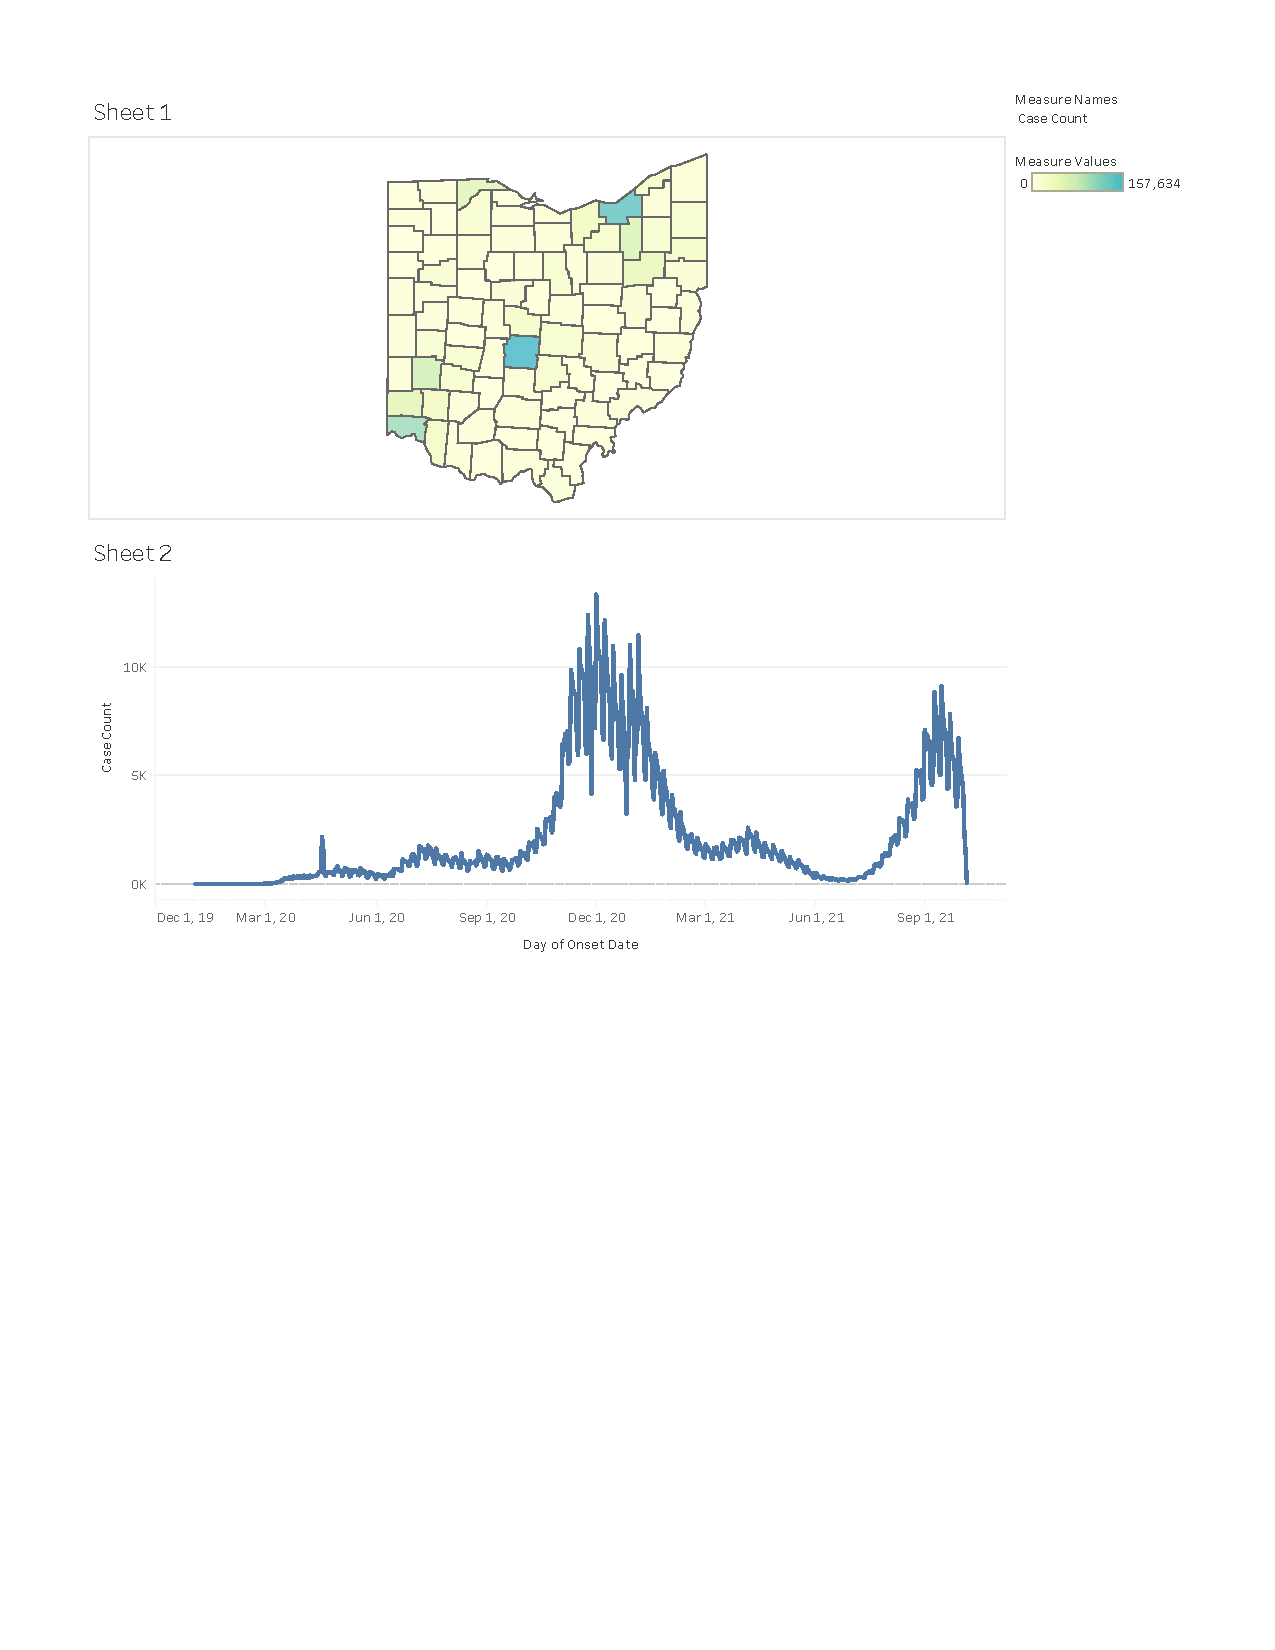
\includegraphics[width=0.8\textwidth,frame, clip, trim={0.5in 4.5in 0.5in 0.5in} ]{../../figures/tableau_example.pdf} 
	
	A schematic, not exact representation, of our Tableau visualizations.
\end{center}



\end{questions}
\end{document}
